% This is LLNCS.DEM the demonstration file of
% the LaTeX macro package from Springer-Verlag
% for Lecture Notes in Computer Science,
% version 2.4 for LaTeX2e as of 16. April 2010
%
\documentclass{llncs}

\usepackage{makeidx}  % allows for indexgeneration
%\usepackage{epsfig}
\usepackage{subfigure}
\usepackage{calc}
\usepackage{amssymb}
\usepackage{amstext}
%\usepackage{amsmath}
%\usepackage{amsthm}
\usepackage{multicol}
%\usepackage{pslatex}
%\usepackage{apalike}
\usepackage{graphicx}
\usepackage{listings}
\usepackage{url}
\newtheorem{observation}{Observation}
\usepackage{zed}
\usepackage{algpseudocode}
\usepackage{hyperref}

%\usepackage[pdftex]{hyperref}
\DeclareGraphicsExtensions{.pdf,.png,.jpg}

\def\composition{{\mathrel{\oplus}}}
\def\optional#1{#1 [0\upto 1]}
\def\Mu{\mu}
\def\ms#1{{#1}}
\def\PA{\ms{PA}}
\def\PC{\ms{PC}}
\def\op{\underline{\smash{{op}}}}
\def\sor{\mathrel{\mathsf{or}}}
\def\orElse{\mathrel{\mathsf{or}}}
\newlength\zedminipagewidth
% we define a set of macros for constants of type 'Kind' 

\def\datamodel{\mathsf{datamodel}}
\def\dataclass{\mathsf{dataclass}}
\def\dataelement{\mathsf{dataelement}}
\def\enum{\mathsf{enum}}
\def\enumeration{\mathsf{enumeration}}
\def\primitivetype{\mathsf{primitivetype}}
\def\datatype{\mathsf{datatype}}
\def\tag{\mathsf{tag}}
\def\dataitem{\mathsf{dataitem}}
\def\abstractitem{\mathsf{abstractitem}}

% and for multiplicity 

\def\optional{0{\upto}1}
\def\mandatory{1{\upto} 1}
\def\many{0{\upto}*}

% partial ordering on constraints

\def\Cimplies{\mathrel{\implies_c}}
\def\Ciff{\mathrel{\iff_c}}

%  partial ordering on text

\def\Timplies{\mathrel{\implies_t}}
\def\Tiff{\mathrel{\iff_t}}

% and conjunction 
\def\Tand{\mathrel{\land_t}}
\def\TAnd{\mathop{\land_t}}
% our globalised version of the defining relations
\def\refines{\mathrel{refines}}
\def\newVersionOf{\mathrel{newVersionOf}}
\def\extends{\mathrel{extends}}
\def\contains{\mathrel{contains}}
% we may have \sqsubseteq and \gg when it comes to analysis 
% our two status values 
\def\draft{\mathsf{draft}}
\def\final{\mathsf{final}}
%load any additional packages

\newcommand\Algphase[1]{%
	\vspace*{-.7\baselineskip}\Statex\hspace*{\dimexpr-\algorithmicindent-2pt\relax}\rule{\textwidth}{0.4pt}%
	\Statex\hspace*{-\algorithmicindent}\textbf{#1}%
	\vspace*{-.7\baselineskip}\Statex\hspace*{\dimexpr-\algorithmicindent-2pt\relax}\rule{\textwidth}{0.4pt}%
}

%\newtheorem{definition}{Definition}
\newcommand{\Lagr}{\mathcal{L}}

%
\begin{document}
	%
	\frontmatter          % for the preliminaries
	%
	\pagestyle{headings}  % switches on printing of running heads
	\title{A Data Modelling Language with Semantics and Provenance}
	
	\author{Jim Davies \and
		David Milward}
	
	\institute{Oxford University, Oxford, U.K.}
	
	
	\maketitle
	
	\begin{abstract}
		An adequate account of data semantics and provenance is important in data management and analysis: to facilitate re-use and help ensure compliance.  This importance increases with the value and the complexity of the data.  This paper introduces a simple data modelling language that can be used also for the capture of semantics and provenance.  It introduces also a toolset, built around the notion of a metadata catalogue, to enable the effective deployment of the language in large organisations and major programmes.  The paper presents a language definition, using the widely-used Eclipse Modeling Framework, together with a design for the catalogue.  It reports on the experience of deploying the language and toolset in two different application domains.
	\end{abstract}
	%
	
	%
	\section{Introduction}
	
	Large organizations tend to have large numbers of data flows within them, some are real-time between different applications or machine actors, which we term \emph{primary data flows} and some are reports, documents and forms which are sent between human actors, these we term \emph{secondary data flows}. Very often business process consists of data flows being transfered and stored on multiple systems and applications, with very little ability to trace or classify what data is being handled.
	
	Abstractions are used in computer science as well as many other disciplines to reason about complex systems, and when systems are designed or reasoned about an abstraction or model will often be used.  Most object oriented software applications are designed with some regard to modelling the key aspects of the application using models and notations such as UML or Ecore.  In the same way most database oriented software applications are constructed using the entity-relationship models. Linked data systems are built using RDF models, and XML dataflows are normally designed using XML Schema. However dataflows can be in many different formats, unstructured text, comma-separated varible files, XML files, binary data standards such as ASTERIX (which is used by Eurocontrol and thus by all air traffic in Europe) and Excel spreadsheets. In both the healthcare and fintech organizations we have looked at Excel is by far the most popular application and format for sending information within the organization and for defining other data formats.
	
	There are tools which are designed to overcome these problems, in particular Enterprise Services Buses (ESB) are used in many organizations to try and achieve interoperability between different services. Such toolkits rely on all participants using a common \emph{service oriented architecture}, and to a point these systems work very well assuming all the software components using the system are configured as services, and use one of the protocols mandated by the toolkit in question.  Our experience in both Healthcare and FinTech indicates that most operational environments ESB technology cover only a relatively small percentage of the dataflows, and that many issues of data provenance and semantics are still present
	
	A Metadata Registry is a toolkit which allows definitions of datasets to be stored, curated and managed. The definitions are metadata, and could be the decription of a field in a relational database, or an element in an XML file. By storing the definitions of every data element and all its relations in a metadata registry the map of all the dataflows in an organization can be created and managed. It is similar to an ESB. an in fact most ESB's have some kind of registy internally to hold metadata. Metadata Registries, such as those conforming to the ISO11179 standard, can help to solve the problem of data incompatibility, provenance and compliance, as is indicated in studies such as those conducted by Ulrich et al. \cite{MDRHL7} . In this study a hybrid architecture consisting of an ISO 11179-3 conformant MDR server application for interactively annotating and mediating data elements and the translation of these data elements into FHIR resources was used to manage data for the North German Tumour Bank of Colorectal Cancer. 
	
	The ISO11179 standard allows complex mapping between data elements, conceptual domains and value domains; however it does not have a mechanism which allows data elements to be easily grouped into hierarchical components, such as are found in most datasets and dataflows. There are two mechanisms defined in ISO11179 for grouping data elements, one is \emph{classifications} and the other is \emph{object properties}, however neither allows for any kind of grouping or componentization of the kind which is found in UML, ERM or XSD. As a result integrating ISO11179 in legacy software systems requires extra work and mapping and therefore many of the issues addressed by the standard are complicated rather than simplified when applying the standard to the design of a metadata registry. 
	
	In this work we have taken the core elements in ISO11179, together with standard model driven engineering principles to build a \emph{metamodel} or \emph{language} specifically for dataset modelling and management in the healthcare sector. We have also applied these principles to different use cases in the fintech sector and found that the same principles apply.
	
	
	\section{Background}
	
	Much of the patient data collected in the U.K.'s National Health Service (NHS) remains unaccessible for medical research. This is because it is held in a variety of commercial software systems which have been built at different times, and have been based on different standards. Reporting consists largely of data being sent in excel spreadsheets, csv files or xml files.  There are over 130 different data models and standards (see TRUD \cite{TRUD2017}) currently being used in the NHS at present, and new ones are being introduced and implemented each year. At present the UK NHS is preparing to implement SNOMED across all systems by 2020, this has largely been achieved in primary care, but has hardly been started in secondary care systems. The main reason for the success in primary care is down to the fact that there are 5 main vendors of primary care systems, all of whom regard the UK primary care market as a critical sector for their business, and hence have been highly motivated to align themselves with core NHS England data management policies..  
	
	In secondary care we see a different picture, the larger hospital trusts are running 2-300 different systems, many of these from vendors with bases outside the UK, who have little incentive to make major changes to for non-critical client sectors. Efforts by the core standards bodies within the NHS to impose standards on hospital trusts have met with partial success. 
	
	In addition to the technical challenges, there are also legal issues imposed by the Health and Social Care Act 2012, NHS Act 2006, the Health and Social Care Act 2012, the Data Protection Act 1998, the Human Rights Act, and the shortly to be introduced General Data Protection Regulations(GDPR).  The complexity of these different legal policies can result in data on a patients other conditions (say liver disease) being withheld from Emergency Care Clinicians when they are performing, for instance, emergency heart surgery. Whilst such legislation clearly is intended to protect the patient's privacy, it can have unforseen side effects not only on the practical aspects of emergency medical care, but also on the ability and ease in which medical data can be aggregated for further research purposes.
	
	It is the medical data that is being stored and aggregated for research purposes that is of interest to this project. Medical data when aggregated is generally stored in relational databases, excel spreadsheets or unstructured pdf and word documents, and querying this data can be very difficult in all these cases. Reports are sent through to the central NHS bodies from local hospital trusts to satisfy reporting requirements in a variety of formats, with no real verification on the data contained within them. There is no question that the information \emph{could} be valuable for research, however extracting data for analysis is very often too costly to perform.  When datasets are prepared for analysis it is often discovered that the structure of the data when stored may not be the same as the structure it is required in now, and there maybe no exact record of how the data was originally recorded. For instance gender may be stored in one system as an enumeration of \emph{yes or no} and in another system as \emph{yes, no, unknown}, if a research writes a query assuming the former they may arrive at incorrect conclusions if the data is actually collected in the format of the latter, but assumed to be conforming to the former. This is an issue of semantics, but it just having a data standard such as HL7 or FHIR does not necessarily solve this problem, we need to be able to record the context in which the data is collected, in this case the version of the standard being used at the time.
	
	The work described here started with the development of an ISO11179 for the CancerGrid project~\cite{davi14}, in this work an ISO11179 metadata registry was built to curate datasets for clinical trials data, and to develop clinical trials software~\cite{davi12}. This work was informed by previous initiatives to implement an ISO11179-compliant registry in the CaBIG initiative, which was used to generate code for web service stubs. One of the problems which emerged from this work was that the ISO11179 standard does not separate abstraction levels for the models and model elements it defines.
	
	When data is aggregated and stored in data warehouses or \emph{data lakes}, it is very often stored in the form in which it was originally collected. For data analysis this can result in two potential problems, it is hardly ever in a form suitable for data analysis, and as was referred to previously, if it does adhere to a standard it may not be possible to find out exactly which version of the standard it complies with. As mentioned earlier the NHS has at least 130 different data standards in use, and ones, such as the NHS Data Dictionary, may have changed 20 or more in the last 15 years. The abstractions used in ISO11179 provide a way of documenting the semantics associated with individual data elements, but there are no suitable abstractions for managing groups of data elements, such as can be easily applied to several different medical datasets, lets say FHIR and SNOMED.
	
	Abstraction is used in mathematics to simplify problems, and arrive at a realistically computable solution for a specific problem. Different abstractions are used for different problems, sometimes these certain abstractions can be applied in many different problem domains. By using the abstractions introduced in the MOD/UML framework and building on this foundation we can arrive at a language and set of rules to automate the way data is collected and made available for analysis.
	
	
	
	\section{Language}
	
	In Model Driven Engineering abstractions are used to define the way models are structured at different abstraction levels, and by applying these concepts to models of datasets we are able to define a metamodel or language which is capable of describing nearly all such datasets. We could arguably do this by using Ecore as it stands, however we are working on the principle, often attributed to Einstein, that one should make \emph{everything as simple as possible but not simpler}. This language for data management is aimed at Information Systems, which are simply storing and handling data. We are not looking at having the language capture \emph{behaviour}, it is a \emph{structural meta-language} for describing data items.
	
	\begin{figure}
		\centering
		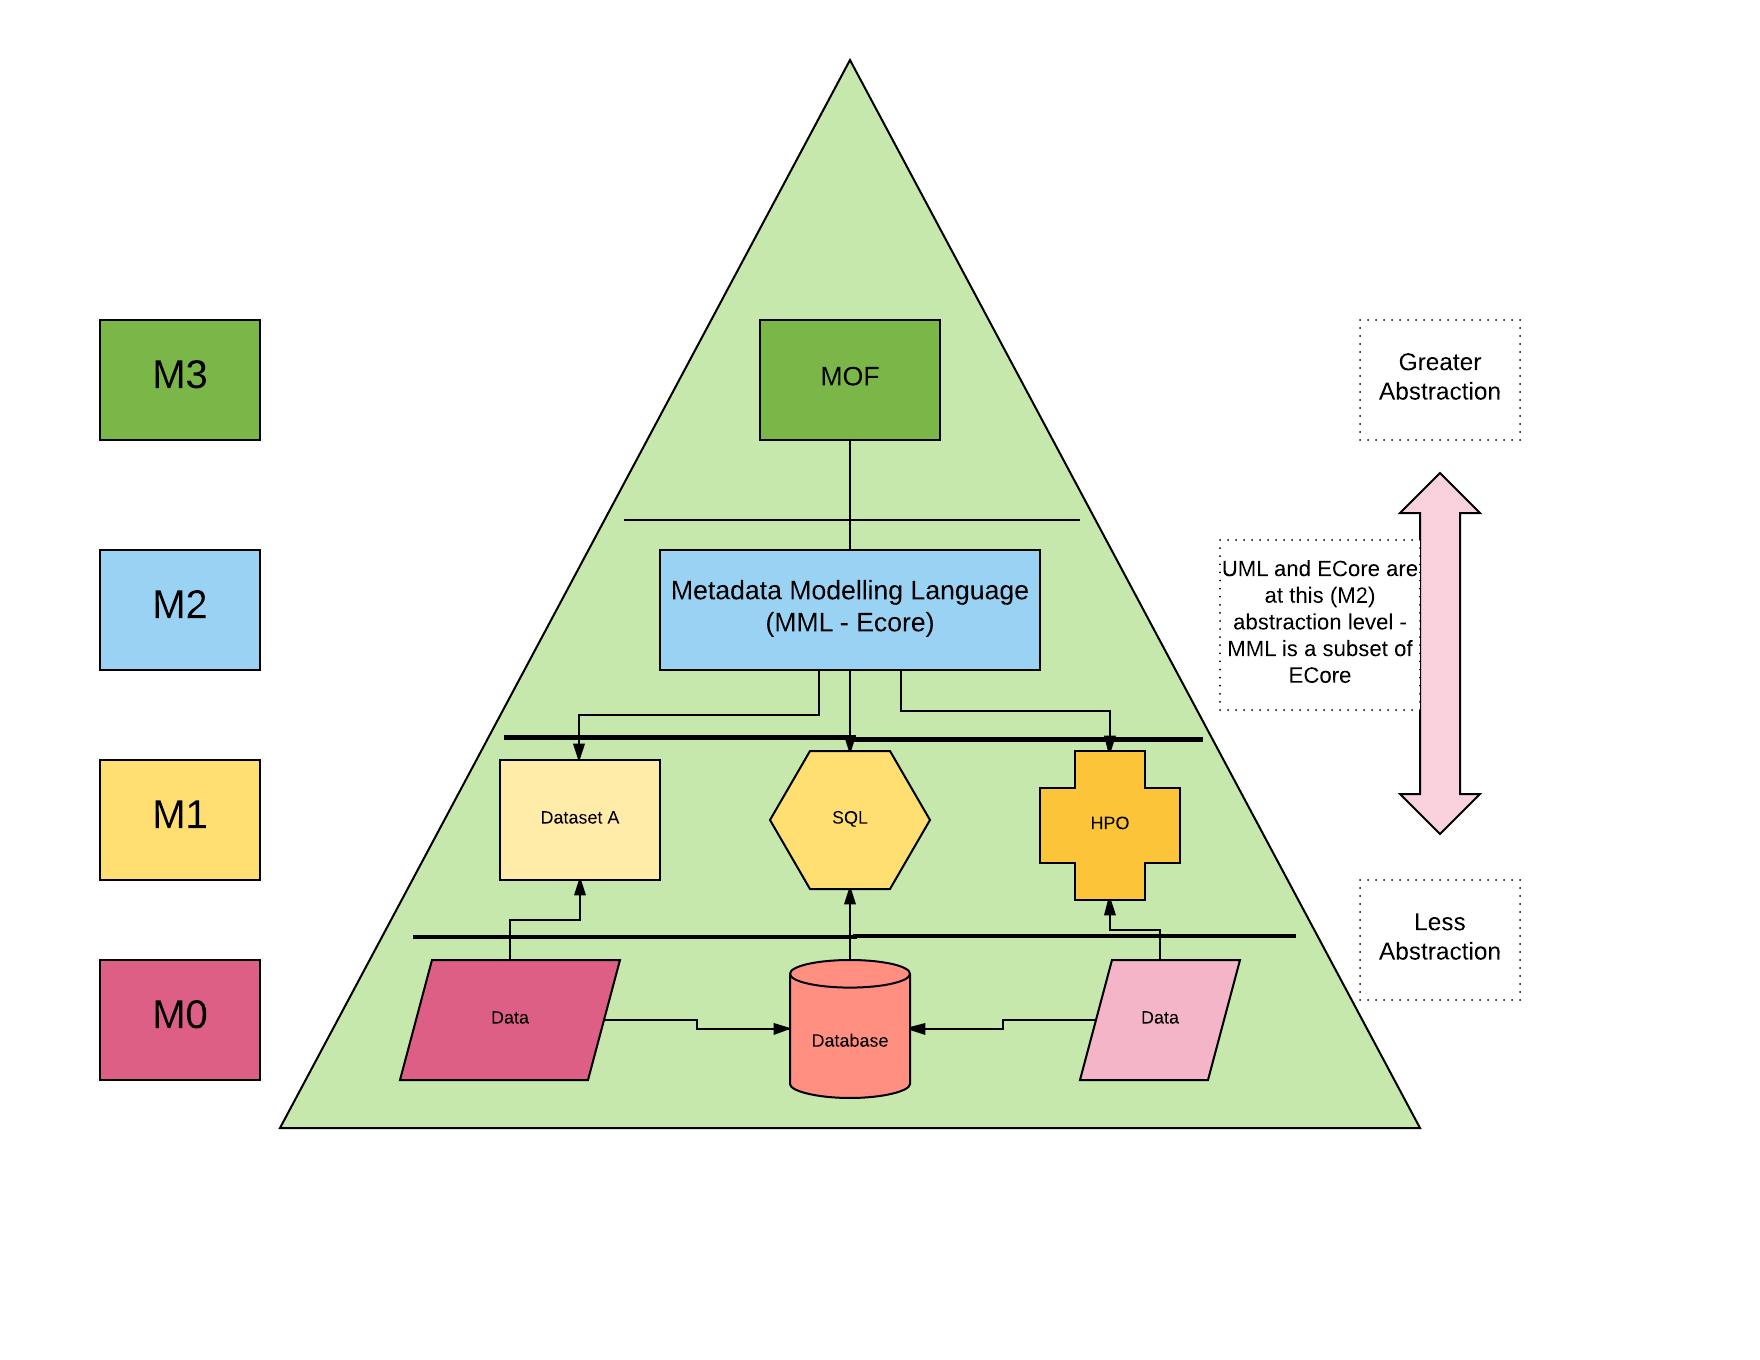
\includegraphics[scale=0.37]{figures/MMLMOFModel}
		\caption{MOF and MML}
		\label{fig:mofmml}
	\end{figure}

	There are two main ways in which MOF uses abstractions, the first is the relationship between MX layers as illustrated in the previous diagram, the second is the notion of \emph{platform independent models} and \emph{platform specific models} which is a notion of abstraction that is applied at the same MOF level. It is this notion that we tie into the idea of \emph{refinement}. We can have a core model, say for Cancer data such as the COSD model, which is defined at the M1 layer as a PIM. It also exists at that layer as an XML model or an Excel spreadsheet, both PSMs, which can be said to \emph{refine} the PIM. 
	
	Ulrich Frank defines~\cite{Frank2013} a set of requirements for building a domain specific modelling language, which we have attempted to follow in designing this metamodelling language for datasets. In short they can be paraphrased and listed as follows:
	\begin{itemize}
		\item A metamodelling language should be supplemented by a metamodelling environment that supports the realization of model editors.
		\item The language concepts used on different levels of abstraction should be clearly separated
		\item The graphic notation should correspond to prevalent graphical notations
		\item The concepts should be supplemented by a language for specifying constraints
		\item The concepts should allow for a clear mapping to concepts used for software development
		\item The language should allow for distinguishing between different levels of abstraction
		\item The language should provide concepts for representing instances
		\item The language should account for dissemination and standardization
	\end{itemize}
	
	Our metamodelling langauge (MML) has a metamodel \textbf{$M_2$} defined at level M2 of MOF. The language can be designated by $\Lagr_{m2}$ and a meta-model ML is formally defined by this language $\Lagr_{m2}$.
	
	Most information systems use a variety of mechanisms to store data, from text files to relational databases, all of which can be modelled at the M1 level.  In fact we can say that the M1 languages which model the data can be designated by $\Lagr_{m1}$, each one defining a Model which we can designate by MI = (mi\_1, mi\_2, ...., mi\_n).  MI being the collection of Models that \emph{conform to} or \emph{implement} MML.  
	
	An example of a \emph{Data Language (say mi\_1)} at this M1 level of abstraction would be the UK NHS's Cancer Outcomes and Services Dataset (COSD) which is a dataset specifying the terminology to use when writing reports on cancer. At present the dataset is defined by both an excel file and an XSD.  Within the NHS there are plenty of other similar datasets, which are used in reports, in databases or by applications.  Whilst MML will not be a fit for every dataset, it is aimed at covering most structural features that occur in datasets, it can be viewed as a subset of Ecore tailored to the domain of data management.
	
	In defining MML we take the notion of a \emph{dataElement} as the core entity in the language, historically it was intended to correspond to a \emph{data element} in ISO11179 and with an \emph{element} in the UML meta-model. It is an atomic data item, capturing one single element that cannot be sub-divided.
	
	The word or stem \emph{abstract} is used in several different ways in this discussion, and the following brief discussion highlights the different usages.  
	
	Firstly we can have an abstract entity which is the implementation of an EClass at the M3 level, that is to say a representation in our language of an EClass which cannot be implemented at the M2 level. It can be \emph{sub-typed} by another EClass at the M2 level and this \emph{sub-class} can be implemented. We use this mechanism to specify both AbstractItem and DataItem as \emph{abstract} entities in our language, however we are not defining an \emph{abstraction} mechanism for MML per se. Later on we will define an inheritance or rather a simple sub-typing mechanism which can be used for \emph{templating} at the M1 model level. 
	
	Secondly we are referring to each layer as being an \emph{abstraction} of the previous layer, and therefore having less concrete description, this is the notion built into the idea of MOF layers. 
	
	
	
	
	
	\subsection{Language Definition}
	
	We need a notion which allows us to group \emph{dataElements} and the obvious notion is the idea of a class, strut or \emph{dataClass}, which is very close the standard notion of a class with no behaviour or operations defined. Above this we need a mechanism for grouping both dataClasses and dataElements, and for this we define the notion of a \emph{dataModel}. 
	
	The notion of a \emph{dataModel} formalises the notion of a dataset, so that we can use the notion of a \emph{dataModel} to standardize and identify a particular version of say, the human phenotype ontology (HPO). 
	
	We may also wish to group \emph{dataModels}, so that we can define a \emph{dataDomain}, which will include perhaps several different models which deal with the same set of concepts. Again we are formalising a set of concepts, at the M2 level of MOF, so that we can apply properties, which we call metadata extensions, across a \emph{dataDomain}. We may for instance wish to formalise a terminology across several different datasets which deal with cancer data, for instance the NHS Data Dictionary, FHIR, COSD and the Genomics England Cancer Model. This is best curated and managed at this level of abstraction, it can then be used at the M1 and M0 level. 
	
	\subsubsection{Core Elements of MML}
	\paragraph{generalElement}
	
	
	\paragraph{DataModel}
	A DataModel is versioning and grouping mechanism for one data-set, it might for instance be a particular database, or a particular XSD Schema which is used in a particular domain, however it allows us to group and version a related set of DataClasses. A DataModel can contain many DataElements, and many DataTypes. A DataModel contains one or more DataItems, which may be implemented as DataClasses, DataElements, DataTypes or EnumerationValues. As all DataItems are also AbstractItems, they can have Tags, which link them to entities outside that DataModel using URI's, and they can have Relationships which are two-way associations with other AbstractItems. DataConstraints are attached to each DataModel and are applicable within that DataModel.
	\paragraph{DataClass}

	A DataClass is a mechanism for grouping DataItems, which are atomic pieces of data. A concept may be represented by a class, but the DataItem is the atomic component of that class, it can't be reduced into any smaller component. A DataClass can be used as a DataItem, in that it can be contained within another DataClass, and so it can be used to provide multi-level grouping within a DataModel. A DataClass can \emph{extend} another DataClass, this \emph{inheritance} mechanism is very straightforward, it allows the child class to have all the member DataItems and DataClasses that are present in the parent. These DataItems and DataClasses are in effect references, so that if the parent class changes then these \emph{inherited} DataItems and DataClasses will be changed as well.
	
	\paragraph{DataElement}
	A DataElement is the smallest data entity described in this langauge, it has a direct one to one relationship with a DataType, since every DataElement will have a corresponding DataType. 
	
	\paragraph{DataType}
	A DataType is a basic type or value representation for a particular DataItem, it represents the kind of unit of the DataItem, for instance for it could be a set of values defined by a enumerations, or it could be a number represented by an integer or double DataType. The notion of DataType here is very similar to that which prevails in the Computer Science world and is defined by Pierce  ~\cite{Pierce} as follows:
	\textbf{A type system is a tractable synthetic method for proving the absence of certain program behaviours by classifying phrases according to the kinds of values they compute}. This corresponds closely, and may be seen as a refined of, the ISO11179 definition of a value domain, which is \textbf{A “data value” is an element of a value domain. “Enumerated value domain” is a value domain that is specified by a list of all its permissible values. a value domain is the set of possible data values of an attribute. } Whilst these definitions differ, for the purposes of developing a physical model for the ISO11179 notion of value domain, the idea of type, as used within UML and Ecore, suffices.
	
	We have defined three different DataTypes all deriving from a parent DataType which itself is derived from the CatalogueElement entity or class. These are a \emph{Primitive} which represents a single primitive value such as a boolean or an integer; and a primitive can also hold information relating to a unit, that is to say a speed may be recorded as an integer, but that DataType may be modified by being an standard unit of measurement. Hence we include two attributes on the Primitive Class to capture these differences. A DataType might be a \emph{ReferenceType}, which is needed if a DataClass is present inside another DataClass, effectively acting as a DataItem, it's type is then the type of the DataClass concerned. 
	
	The last kind of DataType is the \emph{Enumeration} which is a multiple set of ordered key-value pairs, the key-value pairs are part of the \emph{Enum} entity which in turn is derived from the core \emph{CatalogueElement} entity. This enables it to have tags and/or constraints attached to it, which allows terminologies and vocabularies from ontologies to be imported into the language.
	
	\subsection{Identification and Versioning}
	The language uses a notion of identifying artefacts using a \emph{package} namespace notation, so that a DataElement will be part of a DataClass, which is part of a DataModel, which in turn will have unique URI. As an example let's suppose we have a dataset for lung cancer model being curated at oxford, we may use a generic URI for the Oxford Lung Cancer Dataset, something like \emph{http://oxfordcancer.org/lungvx}. This namespace uniquely identifies the lung cancer data model being curated by people using the URI of \emph{http://oxfordcancer.org} as their main identifier. The word \emph{lung} then uniquely identifies the \emph{lung} model, this in turn will contain other DataItems which are DataClasses, DataElement, DataTypes and so forth, each identified by a name, a version number and an artefact type.
	This notion of identification and versioning is a key notion in our language, and is one which enables different datasets to be automatically compared and adjusted for data analysis and possibly data fusion. We require all \emph{generalElements} to be versioned and identified, and since \emph{DataModel}, \emph{DataClass}, \emph{DataElement}, \emph{DataType} and \emph{Relationship} are all derived from \emph{generalElement} they will all have these properties. 
	
	\subsubsection{Relationships}
	
	Having defined the core entities in the language we look at the idea of relationships. Relationships can exist between any \emph{generalElements}, and the common ones are listed below:
	
	\begin{itemize}
		\item ParentChild(Inheritance)
		\item BasedOn(Inheritance)
		\item Supercession
		\item OriginFor
		\item SynonymFor
	\end{itemize}
	
	The first two perhaps need some explanation, the parent-child hierarchy is best illustrated by the \emph{rectangle issue} highlighted in the paper Compositionality and Refinement in Model−Driven Engineering~\cite{SBMF2012}. In the first we are envisaging the sub-typing relationship which is used in most programming languages, whereby the invariants can be relaxed during sub-typing, in the \emph{basedOn} relationship we envisage a situation whereby invariants are strengthen during sub-typing.
	
	
	\subsubsection{Constraints}
	The fact that we are defining a domain specific language based on ECore means that we are able to use OCL as a constraint language, although we can define constraints using first order logic directly. During the building up of a DataClass hierarchy we are able to specify containment relationships, which can be mandatory, optional, alternate, or alternative. We can therefore list a number of relationships and constraints which can be represented using standard logic notation.
	
	\begin{table}
		\caption{Relationships and their logical representation}
		\begin{center}
			\begin{tabular}{r@{\quad}rl}
				\hline
				\multicolumn{1}{l}{\rule{0pt}{12pt}
					Relationship}&\multicolumn{2}{l}{Logical Representation}\\[2pt]
				\hline\rule{0pt}{12pt}
				BasedOn  & \(A \Rightarrow B \)   & \\
				Mandatory.  &  \(C \Rightarrow D\)  & \\
				Alternate  & \(  A \Rightarrow (B_1 \land (\neg B_2 \land ... \land \neg B_n) \lor (B_2 \land (\neg B_1 \land ... \land \neg B_n ) \lor ...  \) & \\[2pt]
			%%	Alternative  & $ P \Rightarrow p_1 \and \not q_2 $ & \\[2pt]
				\hline
			\end{tabular}
		\end{center}
	\end{table}
	
	
	
	
	\subsubsection{MML Grammar}
	
	The following section shows the code used to define the XText grammar, which is used to generate an Ecore meta-model, which in turn is used to define the different datasets used in this project.
	\begin{small}
		\begin{verbatim}
		grammar uk.ac.ox.cs.MML with 
		org.eclipse.xtext.common.Terminals
		
		generate mML "http://www.ac.uk/ox/cs/MML"
		
		MML :
		(elements += AbstractItem)*
		;
		
		
		DataModel:
		'DataModel' name = QualifiedName '{'
		(elements += AbstractItem)*
		'}'
		;
		
		AbstractItem:
		DataModel | DataClass | DataType | Import
		;
		
		QualifiedName:
		ID('.' ID)*
		;
		
		Import:
		'import' importedNamespace = 
		QualifiedNameWithWildcard
		;
		
		QualifiedNameWithWildcard:
		QualifiedName '.*'?
		;
		
		
		DataType:
		'DataType' name = ID
		;
		
		ContainerElement:
		DataClass| DataElement
		;
		
		DataClass:
		'DataClass' name = ID ('extends' superType =
		[DataClass])? '{'
		(dataelements += ContainerElement)*
		'}'
		;
		
		DataElement:
		'DataElement' name = ID ':' type =  
		[DataType|QualifiedName]
		;
		\end{verbatim}
	\end{small}
	
	
	
	\subsection{Language Properties}
	
	
	\section{Application}
	
	
	\subsection{Health Service Example}
	\subsection{FinTech Example}
	
	
	\section{Conclusion}
	\bibliographystyle{splncs}
	\bibliography{CAISE2018}
	
	
	
	
\end{document}


%\bibliographystyle{plain}
%\bibliography{CAISE2bib}



